\documentclass[aspectratio=169]{beamer}

% ---- Visual style, aligned with the provided template ----
\usepackage{xcolor}
\definecolor{HermesOrange}{HTML}{F37021}
\definecolor{SoftBlue}{HTML}{EAF3FF}
\definecolor{SoftGreen}{HTML}{EAF7EF}
\definecolor{SoftRed}{HTML}{FFF0EC}
\definecolor{SoftYellow}{HTML}{FFF7D8}
\definecolor{SoftPurple}{HTML}{F0ECFF}
\definecolor{SoftGray}{HTML}{F6F6F6}
\usetheme{Madrid}
\usecolortheme{seahorse}
\setbeamercolor{structure}{fg=HermesOrange}
\setbeamercolor{frametitle}{bg=HermesOrange!10, fg=black!90}
\setbeamercolor{title}{fg=HermesOrange}
\setbeamercolor{block title}{bg=HermesOrange!15, fg=black!90}
\setbeamercolor{block body}{bg=black!2, fg=black!92}
\setbeamercolor{item}{fg=HermesOrange}
\setbeamertemplate{navigation symbols}{}
\setbeamertemplate{itemize item}{\textcolor{HermesOrange}{$\blacktriangleright$}}
\setbeamertemplate{itemize subitem}{\textcolor{HermesOrange}{$\triangleright$}}

\usepackage{amsmath,amssymb}
\usepackage{array}
\usepackage{booktabs}
\usepackage{tikz}
\usetikzlibrary{arrows.meta,positioning,calc,fit}
\newcommand{\paper}[1]{\textcolor{HermesOrange!90!black}{\textbf{#1}}}
\newcommand{\stlG}{\mathbf{G}}
\newcommand{\stlF}{\mathbf{F}}
\newcolumntype{L}[1]{>{\raggedright\arraybackslash}p{#1}}

\title[Language-Grounded STL Safe RL]{A Staged Plan for Language-Grounded STL Safe RL}
\author{Yuhang Zhang}
\institute{EECS, Washington State University}
\date{\today}

\begin{document}

% ===== 1 =====
\begin{frame}{The Original Problem: Turn a User Command into Safer Behavior}
\begin{block}{Long-term research question}
\large
Can a user describe both a task and a safety requirement in natural language, and can that requirement be translated into STL and used during Safe RL training?
\end{block}

\vspace{0.55em}
\begin{block}{Example command}
\large
``Reach the goal. If you get too close to an obstacle, return to a safe distance within 10 steps.''
\end{block}

\begin{columns}[T]
\column{0.47\textwidth}
\begin{block}{Task objective}
\footnotesize
Reach the goal efficiently.
\end{block}
\column{0.49\textwidth}
\begin{block}{Temporal safety requirement}
\footnotesize
After a warning, recover before a deadline.
\end{block}
\end{columns}
\end{frame}

% ===== 2 =====
\begin{frame}{The Complete Research Chain Has Six Links}
\begin{center}
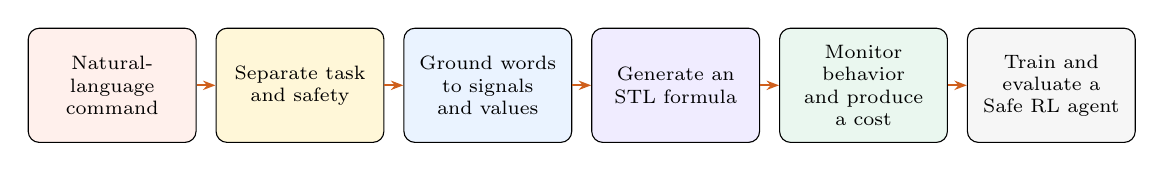
\begin{tikzpicture}[
  stage/.style={draw,rounded corners,align=center,font=\scriptsize,text width=1.78cm,minimum height=1.45cm,inner sep=5pt},
  arr/.style={-{Stealth[length=4.5pt]},thick,HermesOrange!85!black}
]
  \node[stage,fill=SoftRed] (a) {Natural-language command};
  \node[stage,fill=SoftYellow,right=0.24cm of a] (b) {Separate task and safety};
  \node[stage,fill=SoftBlue,right=0.24cm of b] (c) {Ground words to signals and values};
  \node[stage,fill=SoftPurple,right=0.24cm of c] (d) {Generate an STL formula};
  \node[stage,fill=SoftGreen,right=0.24cm of d] (e) {Monitor behavior and produce a cost};
  \node[stage,fill=SoftGray,right=0.24cm of e] (f) {Train and evaluate a Safe RL agent};
  \draw[arr] (a)--(b);
  \draw[arr] (b)--(c);
  \draw[arr] (c)--(d);
  \draw[arr] (d)--(e);
  \draw[arr] (e)--(f);
\end{tikzpicture}
\end{center}

\vspace{0.7em}
\begin{columns}[T]
\column{0.47\textwidth}
\begin{block}{In the example}
\footnotesize
Goal reaching remains the task reward. ``Too close,'' ``safe distance,'' and ``10 steps'' must become measurable conditions.
\end{block}
\column{0.49\textwidth}
\begin{block}{How STL reaches RL}
\footnotesize
The formula is not passed to RL as text. A monitor evaluates the trajectory and converts the result into a safety cost.
\end{block}
\end{columns}
\end{frame}

% ===== 3 =====
\begin{frame}{Each Link Introduces a Different Source of Uncertainty}
\begin{columns}[T]
\column{0.47\textwidth}
\begin{block}{1. Language interpretation}
\footnotesize
Did the system identify the intended task and safety requirement?
\end{block}
\begin{block}{2. Grounding}
\footnotesize
Do words such as ``close'' refer to the correct signal, threshold, and time unit?
\end{block}

\column{0.49\textwidth}
\begin{block}{3. Monitoring and cost design}
\footnotesize
Does the STL monitor judge trajectories correctly, and does its output provide a useful training signal?
\end{block}
\begin{block}{4. Safe RL learning}
\footnotesize
Can the agent reduce temporal safety failures without losing the ability to complete the task?
\end{block}
\end{columns}

\begin{block}{Why the full experiment is difficult to interpret}
\large
Any one component can fail even when the others are correct. An end-to-end failure would not reveal which research problem caused it.
\end{block}
\end{frame}

% ===== 4 =====
\begin{frame}{We Therefore Split the Research into Three Stages}
\begin{center}
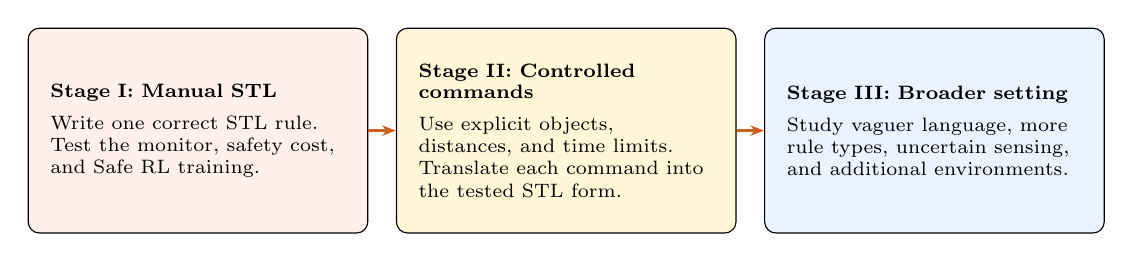
\begin{tikzpicture}[
  phase/.style={draw,rounded corners,align=left,font=\scriptsize,text width=3.75cm,minimum height=2.6cm,inner sep=8pt},
  arr/.style={-{Stealth[length=5pt]},very thick,HermesOrange!85!black}
]
  \node[phase,fill=SoftRed] (a) {\textbf{Stage I: Manual STL}\\[0.45em]
  Write one correct STL rule. Test the monitor, safety cost, and Safe RL training.};
  \node[phase,fill=SoftYellow,right=0.35cm of a] (b) {\textbf{Stage II: Controlled}\\[-0.05em]
  \textbf{commands}\\[0.45em]
  Use explicit objects,\\distances, and time limits.\\Translate each command into\\the tested STL form.};
  \node[phase,fill=SoftBlue,right=0.35cm of b] (c) {\textbf{Stage III: Broader setting}\\[0.45em]
  Study vaguer language, more rule types, uncertain sensing, and additional environments.};
  \draw[arr] (a)--(b);
  \draw[arr] (b)--(c);
\end{tikzpicture}
\end{center}

\vspace{0.6em}
\begin{block}{Current focus}
\large
Stage I isolates the downstream question: if the safety rule is already correct, can it be used effectively in Safe RL?
\end{block}
\end{frame}

% ===== 5 =====
\begin{frame}{Stage I Uses One Concrete Navigation Benchmark}
\begin{columns}[T]
\column{0.44\textwidth}
\begin{block}{Application}
\footnotesize
A simulated mobile robot navigates through a known 2D workspace, reaches a target, and responds when it gets too close to a static hazard.
\end{block}

\begin{block}{Selected benchmark}
\large
\texttt{SafetyPointGoal1-v0}
\end{block}

\column{0.52\textwidth}
\begin{block}{Why this is the first test}
\footnotesize
\begin{itemize}
  \item It already supports goal-directed Safe RL.
  \item Hazard distance can be obtained from simulator state.
  \item Its native hazard cost gives a direct comparison.
  \item Static hazards keep the first experiment easy to interpret.
\end{itemize}
\end{block}
\end{columns}

\begin{block}{Deliberate trade-off}
\footnotesize
This benchmark is less realistic than UAV, driving, or real-robot settings, but it minimizes unrelated engineering and perception uncertainty in the first test.
\end{block}
\end{frame}

% ===== 6 =====
\begin{frame}{Stage I Tests One Bounded-Recovery Rule}
\begin{columns}[T]
\column{0.45\textwidth}
\begin{block}{Rule in plain language}
\large
If the agent enters a warning zone, it must return to a safe distance within \(K\) steps.
\end{block}

\begin{block}{One STL representation}
\normalsize
\[
\stlG\bigl(d_t<d_{\mathrm{warn}}\;\rightarrow\;
\stlF_{[0,K]}(d_t\ge d_{\mathrm{safe}})\bigr)
\]
\footnotesize
Choose \(d_{\mathrm{warn}}<d_{\mathrm{safe}}\); fix all values before training.
\end{block}

\column{0.51\textwidth}
\begin{block}{The experiment in four steps}
\footnotesize
\begin{enumerate}
  \item Define the distance signal and feasible rule values.
  \item Check the rule on clear success and failure paths.
  \item Train agents in the same task with different safety methods.
  \item Compare temporal failures and goal completion.
\end{enumerate}
\end{block}
\end{columns}

\vspace{0.2em}
\begin{center}
\footnotesize
\textbf{Controlled comparison:} keep the environment and task fixed; change only the safety method.
\end{center}
\end{frame}

% ===== 7 =====
\begin{frame}{The Comparison Separates Temporal Safety from Simpler Alternatives}
\small
\begin{tabular}{L{2.55cm} L{3.75cm} L{5.2cm}}
\toprule
\textbf{Method} & \textbf{Advantage} & \textbf{Limitation or role} \\
\midrule
Task reward only & Minimal reference condition & No explicit safety objective \\
\addlinespace
Native hazard cost & Built in and easy to use & Instantaneous; cannot express a recovery deadline \\
\addlinespace
Temporal STL cost & Explicit deadline and reusable monitor & Needs measurable signals, parameters, and a correct monitor \\
\addlinespace
Hand-coded timer & Direct implementation & Useful check, but each new rule needs custom logic \\
\bottomrule
\end{tabular}

\vspace{0.75em}
\begin{block}{Decision to proceed}
\normalsize
Move to Stage II only if the STL rule is measured correctly and reduces recovery failures without an unacceptable loss in goal completion.
\end{block}
\end{frame}

% ===== 8 =====
\begin{frame}{A Successful Stage I Result Has a Narrow, Clear Meaning}
\begin{columns}[T]
\column{0.47\textwidth}
\begin{block}{What the experiment can address}
\footnotesize
\begin{itemize}
  \item Simulated navigation around known static hazards.
  \item Rules based on a directly measurable numeric signal.
  \item Bounded responses: after an event, recover before a deadline.
\end{itemize}
\end{block}

\column{0.49\textwidth}
\begin{block}{What it cannot establish}
\footnotesize
\begin{itemize}
  \item Translation of vague or incomplete language.
  \item Robustness to perception noise, moving hazards, or multiple agents.
  \item Real-world safety or a guarantee of zero violations.
\end{itemize}
\end{block}
\end{columns}

\vspace{0.65em}
\begin{block}{Interpretation}
\large
Success would verify the downstream STL-to-Safe-RL path in one controlled setting. It would justify adding language, not claim that the complete language-based system is solved.
\end{block}
\end{frame}

% ===== 9 =====
\begin{frame}{Stage I Creates a Stable Starting Point for Stage II}
\begin{columns}[T]
\column{0.47\textwidth}
\begin{block}{What Stage I should deliver}
\footnotesize
\begin{itemize}
  \item One fixed navigation task and safety signal.
  \item One tested STL rule and trajectory monitor.
  \item Evidence about whether the temporal cost changes learned behavior.
\end{itemize}
\end{block}

\column{0.49\textwidth}
\begin{block}{What Stage II then adds}
\footnotesize
\begin{itemize}
  \item Controlled commands with explicit distances and deadlines.
  \item A language-to-STL translation component.
  \item Separate evaluation of translation accuracy and downstream behavior.
\end{itemize}
\end{block}
\end{columns}

\begin{block}{Immediate next step}
\large
Freeze a one-page Stage I definition: the task, distance signal, STL rule, initial parameters, and one clear success and failure trajectory.
\end{block}
\end{frame}

\end{document}
